During last years ''irreproducibility'' became a general problem, particularly in Medical-Biosciences where high-dimensionality data are collected from so many different omics to investigate the cellular behaviour, in order to propose new drugs and new patient-oriented treatments.

Due to the analysis complexity and to the not-so-well documented processes, several published papers \cite{Baggerly2009, Potti2011} became a landmark for irreproducibility, leading the scientific community to highlight the weaknesses in reproducing published scientific facts and to promote the \gls{rr}.

The underlying idea of \gls{rr} \cite{Fomel2009b} is to provide public access to analytic data and related analysis code (combined with natural language documentation), in order to allow third-parties to entirely reproduce the findings.

In recent years, many efforts have been spent for sensitizing the scientific community on the relevance of \gls{rr}, such as by producing tools \cite{RussoRighelli2016} supporting reproducible research, by producing scientific works in reproducible research spirit \cite{CostaRighelli2017} or by providing an overview of available methodologies for \gls{rr} \cite{russo2015advantages}.

Anyway, to address \gls{rr} in scientific works many cares are needed during the production of a software or when analyzing data.
As figure \ref{fig:introrr} \cite{Peng2009} shows, the author cannot only make an analysis but need to store all the components needed to a third-party user to reproduce the entire analysis.
To do so, the author needs to give public access not only to the data accompanied but also to the code used to process them, in a ''database-like'' form. 
The ''database-like'' form is required to maintain the reproducibility across the time, which can bring to different code tool versioning.
Moreover, it is fundamental to present the results in the same form as they can be produced with the ''database'' storing the data and the code.

\begin{figure}[H]
\centering
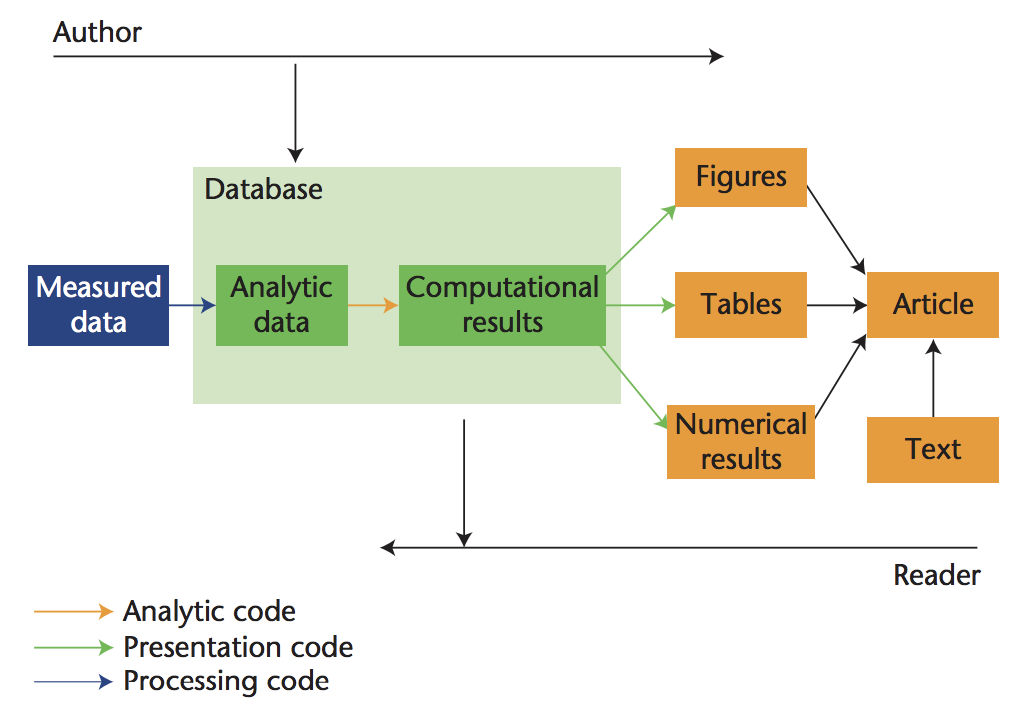
\includegraphics[width=9.5cm, keepaspectratio]{img/intro/rr_scheme.png}
\caption[RR generic scheme]{A scheme of Reproducible Research. (Image from \cite{Peng2009})}
\label{fig:introrr}
\end{figure}

Of course there are several disadvantages trying to respect \gls{rr} constraints, such as the time required not only to analyze the data but also to trace the code and the data in order to give them public access. 
Moreover, nowadays there are several tools  \cite{Aranguren2015, Goecks2010a, Gentleman2004, Shepherd2018}  trying to help implementing \gls{rr} inside the scripts and the tools but it is not so simple which one works better than another, and this can be due to the problem that a standard has not been reached yet.

Fortunately some international journals are starting to require proof of transparency for the proposed works which include computational analysis.
This is advantageous because from one side is leading the scientific community to propose always easier solutions for using tools for \gls{rr}, and from another side the analysts are ''forced'' to release their data and code to demonstrate transparency and, consequently, more robust findings.

Unfortunately, despite all efforts of \gls{rr} community, the Life Science society is still far from a standard for reproducibility \cite{Iqbal2016}, showing that the way is still long to be covered.


